\chapter{Theoretical Work Background}

\section{Introduction}
\label{sec:intro}
Artificial intelligence (AI) has become indispensable in medical imaging, offering tools that can assist—and in some cases outperform—radiologists in detecting and characterizing pathologies. In the context of brain tumors, AI-driven methods enable rapid and accurate identification of tumor boundaries and grading, directly impacting treatment planning and patient outcomes.

In this chapter, we lay the theoretical groundwork for our hybrid approach to brain tumor analysis. We begin with the fundamentals of digital image processing in medical contexts, then review classical machine-learning methods such as Support Vector Machines (SVM). Next, we introduce deep learning, focusing on convolutional neural networks (CNNs) and their encoder–decoder variants, culminating with the U-Net architecture that underpins our segmentation stage. Along the way, we discuss key concepts—loss functions, optimization, regularization, and evaluation metrics—that guide the design and assessment of both our segmentation and classification models.


\section{What Is Artificial Intelligence?}

Artificial Intelligence (\glsxtrshort{ai}) is a multidisciplinary field focused on developing machines and computer programs capable of performing tasks that typically require human intelligence, such as visual perception, reasoning, decision making, and language understanding. According to \cite{sciencedirect_ai_overview}, AI is defined as:

\begin{quotation}
  the science and engineering of creating intelligent machines, particularly intelligent computer programs that can perform tasks requiring human intelligence, such as visual perception, decision making, and language translation.
\end{quotation}

In other words, AI includes both the study of human cognition—how people perceive, learn, reason, and decide—and the development of algorithms and systems that can perform tasks requiring “intelligence,” such as visual recognition or decision making. While some AI techniques draw inspiration from biological processes (e.g. neural networks), the field also embraces purely mathematical and statistical methods.

\begin{figure}[H]
  \centering
  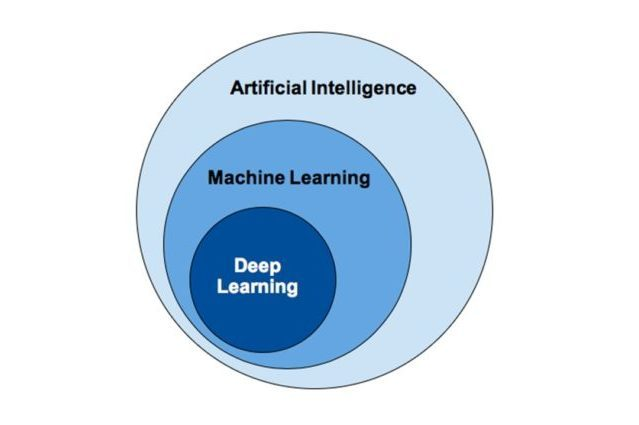
\includegraphics[width=0.6\textwidth]{Images/Chapter1/ai.jpg}
  \caption{Relationship between AI, machine learning, and deep learning.}
  \label{fig:ai}
\end{figure}

\section{Machine Learning}
\label{sec:ml}
Machine learning (\glsxtrshort{ml}) has emerged as a crucial area of study for organizations aiming to harness data resources and gain deeper insights into their operations. Unlike traditional programming methods, where explicit instructions are coded, machine learning enables systems to learn directly from data. In the medical imaging field, ML techniques offer powerful ways to analyze complex MRI data, supporting more accurate and efficient diagnostic processes. However, machine learning is a complex process that involves using diverse algorithms to iteratively learn from data, refine data representations, and make predictions. By feeding training data into these algorithms, increasingly accurate models can be developed. These machine learning models represent the knowledge acquired by algorithms during the training phase \cite{hurwitz2018mlfd}.

\begin{figure}[H]
  \centering
  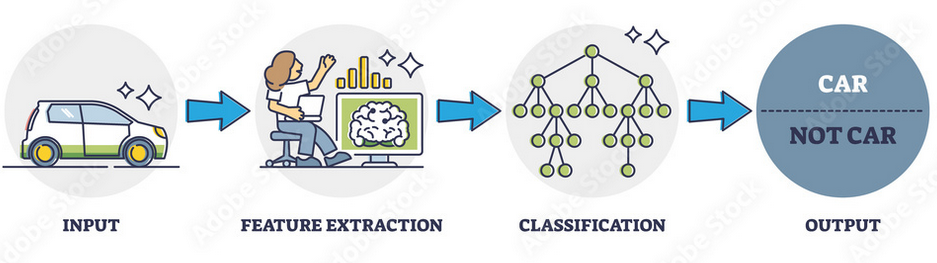
\includegraphics[width=0.8\textwidth]{Images/Chapter1/ml.png}
  \caption{Machine learning process.}
  \label{fig:ml}
\end{figure}
\subsection{Machine Learning approachs}
\subsubsection{Supervised Learning}
In supervised learning, the algorithm learns from labeled training data, where each data point is associated with a corresponding label or target value as depicted in Figure \ref{fig:superml}. Examples of supervised learning algorithms include linear regression , decision trees , random forests , support vector machines , and neural networks.

\begin{figure}[H]
  \centering
  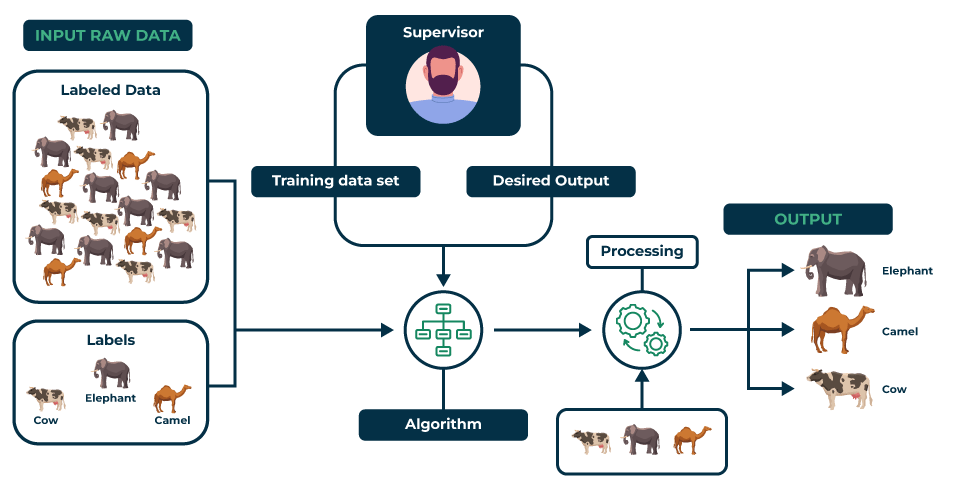
\includegraphics[width=0.8\textwidth]{Images/Chapter1/superml.png}
  \caption{Supervised learning process.}
  \label{fig:superml}
\end{figure}

\subsubsection{Unsupervised Learning}
Unsupervised learning deals with unlabeled data, where the algorithm learns to find patterns or
structure in the data without any specific guidance. Such as k-means and hierarchical
clustering, and dimensionality reduction techniques, such as principal component analysis
and t-distributed stochastic neighbor embedding,  Figure \ref{fig:unsuperml}
\begin{figure}[H]
  \centering
  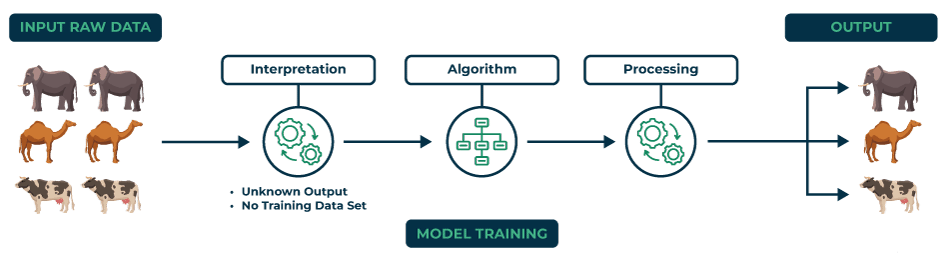
\includegraphics[width=0.8\textwidth]{Images/Chapter1/unsuperml.png}
  \caption{Unsupervised learning process.}
  \label{fig:unsuperml}
\end{figure}

\subsubsection{Reinforcement Learning}
Reinforcement learning is a type of machine learning where an agent learns to make decisions by interacting with an environment. The agent receives feedback in the form of rewards or penalties based on its actions, allowing it to learn optimal strategies over time. This approach is often used in robotics, game playing, and autonomous systems. Figure \ref{fig:reinforcement} illustrates the reinforcement learning process.
\begin{figure}[H]
  \centering
  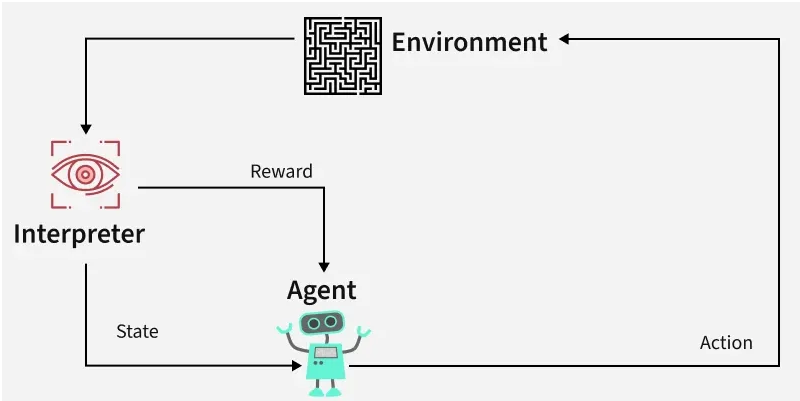
\includegraphics[width=0.8\textwidth]{Images/Chapter1/reinforcement.png}
  \caption{Reinforcement learning process.}
  \label{fig:reinforcement}
\end{figure}

\subsection{Support Vector Machines (SVM)}
\label{sec:svm}
Support Vector Machines (SVMs) are supervised machine learning models widely used for classification and regression tasks. The core idea of SVM is to find an optimal hyperplane that separates data points of different classes with the maximum possible margin, which enhances the model’s ability to generalize to unseen data. SVMs can efficiently handle both linear and non-linear classification problems by employing the kernel trick, which implicitly maps input data into a higher-dimensional feature space where a linear separation becomes possible. The theoretical foundation of SVMs is based on the Structural Risk Minimization (SRM) principle, which aims to minimize an upper bound on the generalization error, offering advantages over traditional Empirical Risk Minimization approaches. Originally developed by Vapnik and colleagues in the 1990s, SVMs have become popular due to their strong empirical performance and robustness to overfitting, especially in high-dimensional spaces \cite{Gunn1998SupportVM}.
\begin{figure}[H]
  \centering
  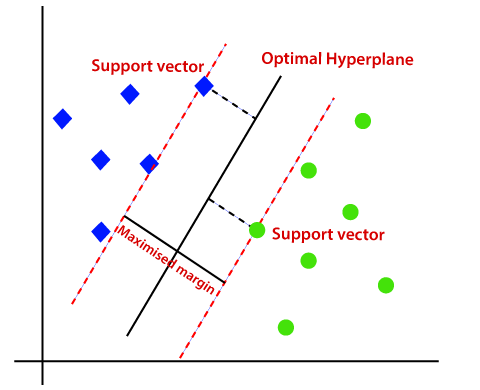
\includegraphics[width=0.4\textwidth]{Images/Chapter1/svm.png}
  \caption{Support Vector Machine.}
  \label{fig:svm}
\end{figure}
The fundamental formula defining the decision boundary of a Support Vector Machine (SVM) is a hyperplane expressed as:
\begin{equation}
  \mathbf{w}^\top \mathbf{x} + b = 0
\end{equation}
where $\mathbf{w}$ is the weight vector normal to the hyperplane, $\mathbf{x}$ is the input feature vector, and $b$ is the bias term.

For binary classification with labels $y_i \in \{+1, -1\}$, the SVM enforces the following constraints on each training point $(\mathbf{x}_i, y_i)$:
\begin{equation}
  y_i \bigl(\mathbf{w}^\top \mathbf{x}_i + b\bigr) \;\ge\; 1,
  \quad \forall\,i.
\end{equation}

The margin width (the distance between the closest points of each class to the hyperplane) is given by $\tfrac{2}{\|\mathbf{w}\|_2}$.  Maximizing this margin is therefore equivalent to minimizing $\|\mathbf{w}\|_2$, leading to the following convex optimization problem:

\begin{align}
  \min_{\mathbf{w},\,b} \quad & \frac{1}{2} \|\mathbf{w}\|_2^2,                             \\
  \text{subject to} \quad     & y_i \bigl(\mathbf{w}^\top \mathbf{x}_i + b\bigr) \;\ge\; 1,
  \quad \forall\,i.
\end{align}

For non-linearly separable data, slack variables and kernel functions can be introduced, but the core formulation remains centered on maximizing the margin around this hyperplane.

\section{Deep Learning}
\label{sec:dl}
Deep learning has emerged as a powerful approach for modeling complex data through intricate architectures that incorporate non-linear transformations. Neural networks, including deep neural networks, serve as the fundamental components of deep learning. These techniques have achieved remarkable progress in various domains such as sound and image processing, enabling tasks like facial recognition, speech recognition, computer vision, language processing, and text classification. The potential applications of deep learning are vast and continue to expand.

Different types of neural network architectures, such as multilayer perceptrons, Convolutional Neural Networks (\glsxtrshort{cnn}s), and recurrent neural networks, cater to specific data types and tasks. These architectures are characterized by deep layers organized in a cascading manner. Successful implementation of deep learning requires well-designed stochastic optimization algorithms, appropriate initialization techniques, and thoughtful structure selection.

\begin{figure}[H]
  \centering
  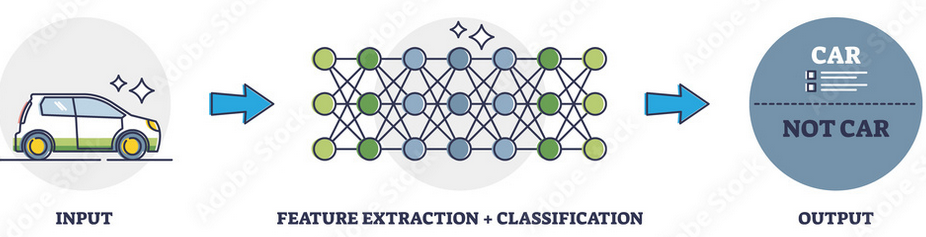
\includegraphics[width=0.8\textwidth]{Images/Chapter1/dl.png}
  \caption{Deep learning process.}
  \label{fig:dl}
\end{figure}

\subsection{Convolutional Neural Networks (CNNs)}
\label{sec:cnn}
A convolutional neural network (CNN) is a type of neural network with a topology similar to a grid, inspired by the human brain. It is commonly used for image processing tasks, as well as natural language processing.

A CNN consists of two main parts. The input is an image, represented as a 2D matrix of pixels for grayscale images and a 3D matrix of pixels for color images (Red, Green, Blue).

The first part of a CNN is the convolutional layer, which acts as a feature extractor. The image is passed through a series of filters, or convolution kernels, to generate new images called feature maps. Some intermediate filters reduce the image resolution. Finally, the feature maps are concatenated to form a vector of features, known as the CNN code.

The output of the convolutional layer, the CNN code, is the input to the second part of the network. The main role of this part is to combine the features of the CNN code to classify the image. The output is a final layer with one neuron per category.
\begin{figure}[H]
  \centering
  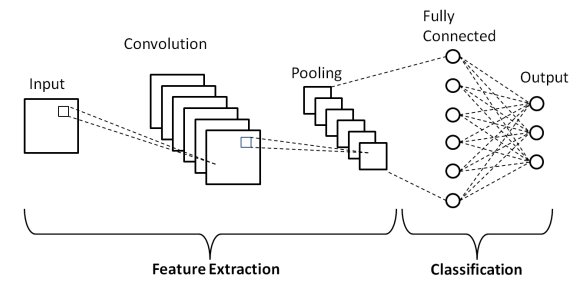
\includegraphics[width=0.8\textwidth]{Images/Chapter1/cnn.png}
  \caption{Convolutional Neural Network.}
  \label{fig:cnn}
\end{figure}

\subsubsection{Convolutional Layer}
\label{sec:conv}

The convolutional layer is the most important layer and usually the first layer in a CNN. It consists of three main elements involved in the convolution operation:
\begin{itemize}
  \item \textbf{Input image} ($f$)
  \item \textbf{Feature detector (filter)} ($h$)
  \item \textbf{Feature map (output)} ($G$)
\end{itemize}

A convolution takes an image and a filter as input and applies the convolution operation to produce a new image, called the activation map or feature map.

The activation map values are calculated using the following formula:
\begin{equation}
  G[m,n] \;=\; (f * h)[m,n]
\end{equation}
where
\begin{itemize}
  \item $f$ is the input image,
  \item $h$ is the convolution filter,
  \item $m,n$ are the spatial indices over which the convolution is computed.

\end{itemize}
\begin{figure}[H]
  \centering
  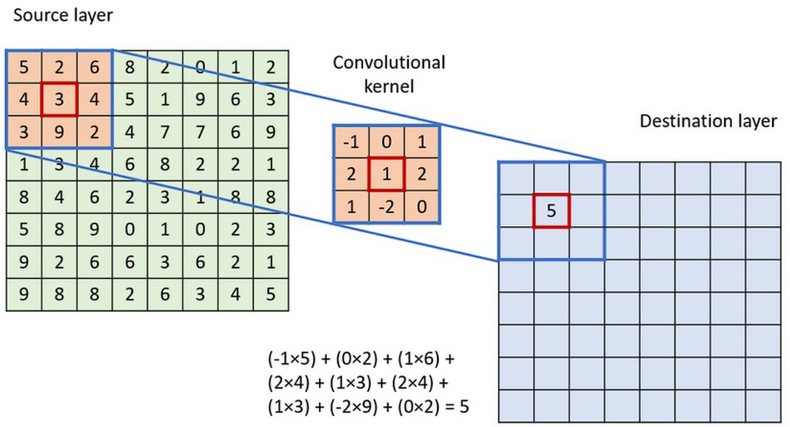
\includegraphics[width=0.6\textwidth]{Images/Chapter1/conv.png}
  \caption{Convolution Layer.}
  \label{fig:conv}
\end{figure}

\subsubsection{Correction Layer (ReLU)}

The Correction Layer, typically implemented using the Rectified Linear Unit (ReLU), is an activation function applied after each convolution operation to enhance processing efficiency. It replaces all negative pixel values with zero, introducing non-linearity into the network while maintaining computational simplicity. The ReLU function is defined as:

\begin{equation}
  f(x) = \max(0, x)
\end{equation}

Several other activation functions exist, such as the sigmoid function, the hyperbolic tangent function (tanh), and the hyperbolic saturating tangent function. However, ReLU is often preferred in deep learning models because it enables faster convergence and better performance compared to these alternatives.

\subsubsection{Pooling Layers}

Pooling layers are utilized to reduce the spatial dimensions of feature maps while preserving the most important information and features. This helps decrease computational complexity and mitigate overfitting. There are several types of pooling operations:

\begin{itemize}
  \item \textbf{Max Pooling}:
        It selects the maximum value from each patch of the feature map. Typically, a $2 \times 2$ patch is used. Max pooling is the most commonly used pooling method.

  \item \textbf{Min Pooling}:
        The inverse of max pooling; it selects the minimum value from each patch of the feature map.

  \item \textbf{Average Pooling}:
        It computes the average of all the values within each patch of the feature map by summing the values and dividing by the number of elements.

  \item \textbf{Sum Pooling}:
        It computes the sum of all elements within each patch of the feature map.

  \item \textbf{Flattening}:
        After the pooling operations, the resulting feature maps are flattened into a single one-dimensional vector to prepare for fully connected (dense) layers.
\end{itemize}

\subsubsection{Fully Connected Layer}

after the convolution and pooling layers, the high-level reasoning in the neural network is done in fully connected layers. The output of flattening is the input of FC layers which are the same as artificial neural networks and carry out the same mathematical operations. The last fully-connected layer uses an activation function such as sigmoid or softmax to get probabilities of the outputs.

\subsection{U-Net Architecture}
U-Net is a convolutional neural network architecture specifically designed for biomedical image segmentation. Introduced by Ronneberger et al. in 2015, U-Net features a symmetric encoder-decoder structure: the contracting path (encoder) captures image context through successive convolution and pooling operations, while the expansive path (decoder) enables precise localization via upsampling and concatenation with high-resolution features from the encoder. This architecture allows U-Net to achieve accurate segmentation even with limited annotated data by leveraging extensive data augmentation. U-Net has demonstrated superior performance in various biomedical segmentation challenges, notably outperforming previous methods in tasks such as neuronal structure segmentation in electron microscopy images and cell tracking in light microscopy \cite{ronneberger2015u}.

\begin{figure}[H]
  \centering
  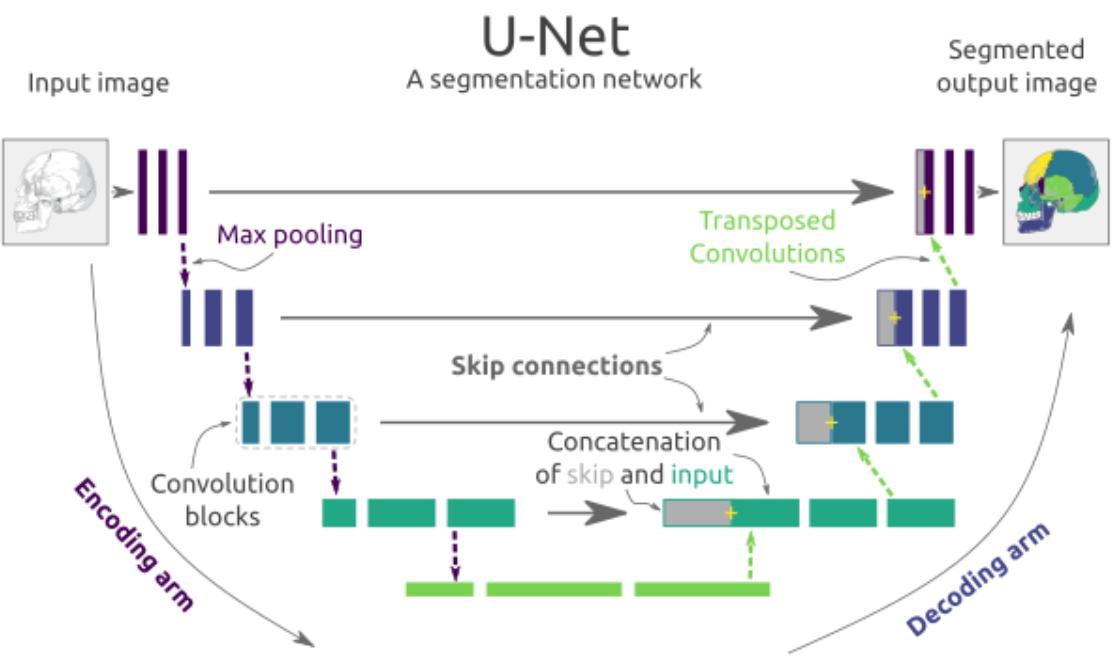
\includegraphics[width=0.8\textwidth]{Images/Chapter1/unet2.png}
  \caption{U-Net Architecture.}
  \label{fig:unet}
\end{figure}

\subsubsection{Key Components of a U-Net Architecture}

\begin{itemize}
  \item \textbf{Contracting Path (Encoder):} \\
        This path is responsible for extracting contextual features from the input image. It consists of repeated blocks of two $3\times3$ convolutional layers (with ReLU activation), followed by a $2\times2$ max pooling operation for downsampling. With each downsampling step, the number of feature channels is doubled, allowing the network to capture increasingly abstract representations of the input.

  \item \textbf{Bottleneck:} \\
        Located at the deepest part of the network, the bottleneck consists of convolutional layers without pooling. It serves as the bridge between the encoder and decoder, capturing the most condensed and abstract features of the input.

  \item \textbf{Expansive Path (Decoder):} \\
        This path reconstructs the spatial resolution of the feature maps and enables precise localization. Each step in the decoder involves upsampling the feature map (often via transposed convolution or up-convolution), concatenating it with the corresponding feature map from the encoder (skip connection), and then applying two $3\times3$ convolutions (with ReLU activation). The number of feature channels is halved at each upsampling step.

  \item \textbf{Skip Connections:} \\
        At each level, feature maps from the encoder are concatenated with the upsampled feature maps in the decoder. These skip connections help retain high-resolution spatial information that might otherwise be lost during downsampling, improving the accuracy of segmentation boundaries.

  \item \textbf{Final Output Layer:} \\
        The last layer is typically a $1\times1$ convolution that maps each feature vector to the desired number of output classes, producing a pixel-wise classification map for segmentation tasks.
\end{itemize}

This U-shaped design enables U-Net to effectively combine global context with fine-grained localization, making it highly effective for precise image segmentation tasks.

\subsection{Megnatic Resonance Imaging (MRI)}
\label{sec:mri}
Magnetic resonance imaging (MRI) uses a powerful magnetic field and radio waves to
generate detailed and high-resolution images of organs and tissues inside the human body, as
depicted in Figure \ref{fig:mri}. This non-invasive imaging method offers significant advantages in
visualizing intricate details of the brain, spinal cord, joints, and soft tissues. MRI plays a vital
role in diagnosing and evaluating a wide range of medical conditions, such as tumors,
neurological disorders, and musculoskeletal injuries. Its ability to produce precise and detailed
images aids healthcare professionals in accurately identifying and assessing these conditions,
enabling effective treatment planning and optimal patient care \cite{verywell_mri}.

\begin{figure}[H]
  \centering
  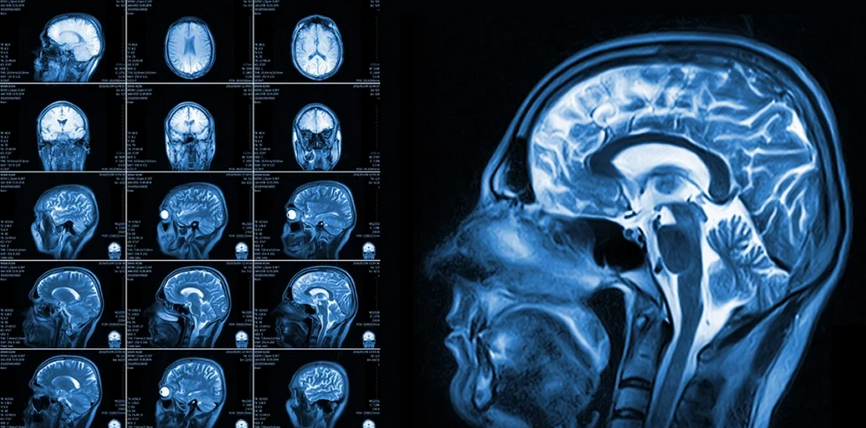
\includegraphics[width=0.6\textwidth]{Images/Chapter1/mri.png}
  \caption{Magnetic Resonance Imaging (MRI).}
  \label{fig:mri}
\end{figure}

\section{Conclusion}
\label{sec:conclusion}

In this chapter, we established the theoretical foundation necessary for our study on brain tumor analysis using artificial intelligence techniques. We first explored the fundamental concepts of artificial intelligence, machine learning, and deep learning, emphasizing their significance in the medical imaging domain. We discussed the various machine learning approaches, highlighting the principles and applications of Support Vector Machines (SVMs) for classification tasks. Furthermore, we introduced deep learning methodologies, focusing on Convolutional Neural Networks (CNNs) and their components, including convolutional, pooling, and fully connected layers. Finally, we presented the U-Net architecture, a specialized CNN model for biomedical image segmentation, which plays a crucial role in the segmentation phase of our proposed hybrid approach. This theoretical background sets the stage for the practical implementation and evaluation of our models in the following chapters.
